\section{Entwurf der Kommunikationskomponente}
Die zweite Komponente des Systems ist für die Kommunikation mit einem Desktop-PC verantwortlich. Unter die Kommunikationsaufgaben fällt einerseits die Übermittlung relevanter Daten des Regelkreises, wie z.B. der aktuelle Wert des Zustandvektors. Andererseits nimmt die Kommunikationskomponente Steuerbefehle entgegen und leitet diese an die Regelungskomponente weiter. Dadurch können während der Ausführung der Anwendung Konfiguration der Versuche durchgeführt werden. Beispiele hierfür sind die Auswahl des zu verwendeten Regler- oder Filterkonzeptes. Für die Verbindung zwischen der Ziel- und Entwicklungsplattform wird das TCP/IP-Protokoll verwendet, wobei die BeagleBone Black-Anwendung als Server fungiert.

Der Kontrollfluss der Kommunikationskomponente wird ebenfalls als Zustandsmaschine modelliert. Diese besitzt die beiden Zustände \textit{Standby} und \textit{Running}. Im Zustand \textit{Standby} wartet der TCP/IP-Server auf die Verbindungsanfrage eines Clients. Ein Verbindungsaufbau wird durch ein entsprechendes Event signalisiert, woraufhin die Zustandsmaschine in \textit{Running} wechselt. In diesem Zustand werden Nachrichten der Regelungskomponente an den Client und umgekehrt von dem Client an die Regelungskomponente weitergeleitet. Der Verbindungsabbruch durch den Client wird wiederum durch ein Event signalisiert. Daraufhin kehr die Zustandsmaschine in \textit{Standby} zurück und wartet auf eine erneute Verbindungsanfrage.
\begin{figure}[h!]
\centering
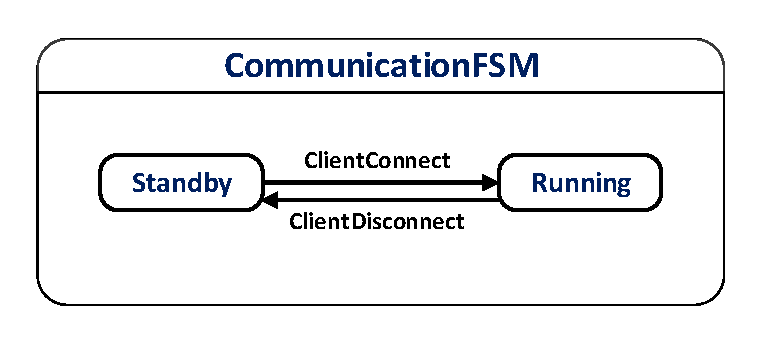
\includegraphics[width=0.7\linewidth]{img/SW_4_CommComp_SC.pdf}
\caption{Zustandsdiagramm der Kommunikations-Komponente, Quelle: eigene Darstellung}
\end{figure}
Für die Implementierung der Zustandsmaschine wird die objektorientierte Methode nach Samek verwendet (Abschnitt...). An dieser Stelle werden keine Templates verwendet, da die Maschine lediglich zwei Unterstände besitzt. Des weiteren ist nicht zu erwarten, dass sich das Zustandsdiagramm im Entwicklungsprozess verändert.

Der Actionhandler der Zustandsmaschine besitzt eine Instanz der Klasse \textit{CServer}, welche die nötigen Serverfunktionalitäten bereitstellt.
\begin{lstlisting}
class CServer
{
public:
	void init();
	bool waitForClient();
	bool transmitMessage(CMessage& msg);
	bool receiveMessage(CMessage& msg);
	...
};
\end{lstlisting}
In der \textit{waitForClient()}-Methode wird der aufrufende Thread blockiert bis ein Client eine Verbindung aufbaut. Anschließend können mittels der Methoden \textit{transmitMessage()} und \textit{receiveMessage()} Nachrichten versendet bzw. empfangen werden. Da es sich bei einer TCP/IP-Verbindung um einen Bytestream handelt wird der Typ \textit{CMessage} als Datenpaket in der Übertragung verwendet. Das heißt das lediglich Instanzen von \textit{CMessage} übermittelt werden, wobei die Objekte byteweise versendet und empfangen werden. Im Anschluss werden die einzelnen Bytes wieder zu einer Instanz von \textit{CMessage} zusammengesetzt.

Da das Versenden und Empfangen von Nachrichten parallel erfolgen soll, wird die Kommunikationskomponente um einen zweiten Thread erweitert. Dieser wird in der Klasse \textit{CReceiveTask} implementiert, welche von \textit{IRunnable} erbt. Dieser Thread ist sowohl für das Empfangen von Nachrichten als auch die Annahme von Verbindungsanfragen zuständig.
\begin{lstlisting}
void CReceiveTask::run()
{
	while(true)
	{
		if(mServer.waitForClient() == true)
		{
			sProxy.clientConnected();
		}
		
		CMessage receivedMsg;
		while(mServer.receiveMessage(receivedMsg)
		{
			sProxy.routeClientMessage(receivedMsg);
		}
		sProxy.clientDisconnect();
	}
}
\end{lstlisting}
Der Thread ruft zunächst die \textit{waitForClient()}-Methode der \textit{CServer}-Instanz auf, welche den Thread solange blockiert bis eine Verbindung aufgebaut wurde. Daraufhin erzeugt der Task mittels des Proxy ein Ereignis um die Komponente zu benachrichtigen. Im nächsten Schritt ruft der Task die \textit{receiveMessage()}-Methode des Servers in einer Schleife auf. Diese blockiert den Thread bis entweder eine Nachricht eintrifft oder die Verbindung abgebrochen wird. Die Fallunterscheidung erfolgt mit Hilfe des Rückgabewertes von \textit{receiveMessage()}, wobei im Fall einer empfangenen Nachricht diese über den Proxy an die Regelungskomponente weitergeleitet wird. Wird die Verbindung von dem Client abgebrochen verlässt der Task die Empfangsschleife. Anschließend wird der Verbindungsabbruch über den Proxy signalisiert und wieder auf eine erneute Anfrage gewartet.

Der Hauptthread der Komponente wird über deren Eventqueue synchronisiert. Hierbei sind lediglich drei Fälle zu unterscheiden. Die Events \textit{ClientConnect} und \textit{ClientDisconnect} führen jeweils zu einem Zustandswechsel der Zustandsmaschine. Befindet diese sich im Zustand \textit{Running} wird zusätzlich geprüft ob es sich um eine Nachricht handelt, welche über den Server an den Desktop-Client weitergeleitet werden muss.